% !TEX program  = xelatex
\documentclass[a4paper]{article}
\usepackage{amsmath}
\usepackage{amssymb}
\usepackage{enumerate}
\usepackage{amstext}
\usepackage{ctex}
%\usepackage{braket}
\usepackage[european]{circuitikz}
\usepackage{multirow}
\usepackage{graphicx}
\usepackage{subfig}
\usepackage{float}
\usepackage{url}
%\usepackage[table,xcdraw]{xcolor}
\usepackage{colortbl}
\usepackage{geometry}
\geometry{left=2.5cm,right=2.5cm,bottom=2.5cm,top=2.5cm}

\title{模电实验报告11:有源RC滤波电路实验}
\author{xy\quad 学号\quad 匡亚明学院}
\date{2019年2月29日}
\begin{document}
\maketitle
\bibliographystyle{unsrt}
%--------main-body------------

\section{实验目的}
\begin{enumerate}
\item 学习使用运放组成RC低通、高通、带通和带阻滤波电路的二阶基本节。了解高阶RC滤波器的组成和性能。
\end{enumerate}

\section{实验仪器}
示波器、信号发生器、交流毫伏表、数字万用表。

\section{预习内容}
\begin{enumerate}
\item 复习关于使用运放组成RC低通、高通、带通和带阻滤波电路的二阶基本节方面的知识。
\item 定性绘制本实验所用电路的幅频特性曲线和相频特性曲线。
\end{enumerate}

\section{实验内容}
当对滤波器要求不高时,往往使用一阶基本节或二阶基本节。当对滤波器要求较高时,就需要使用高阶滤波器。高阶滤波器通常由一阶基本节和/或二阶基本节组成。

低通二阶基本节的传递函数通常写成规范形式(即(\ref{eq2})式)。可实现这一传递函数的电路是多种多样的。高通、带通和带阻二阶基本节亦然。本实验选用了有限正增益低通二阶基本节电路。
大多数现有教科书在RC有源滤波器设计中,其R、C参数是在运放为理想运放的假设下计算出来的。所以,实际电路的幅频特性曲线和相频特性曲线与理想的幅频特性曲线和相频特性曲线常常会有差别。而这种差别往往随着滤波器的理论设计性能指标越高而变得越大。由于在有限正增益低通二阶基本节电路中,运放仅用于组成有限增益放大器,所以,在实际电路中由“理想运放”假设引起的差别很小。

由(\ref{eq2})式可见,低通二阶基本节电路的传递函数只有三个参数,即$A_o$、$\omega_L$、$Q_L$,因此,最少只要有三个RC元件和一个运放就可构成一个二阶基本节电路。通常,二阶基本节电路的元件个数都大于3。一般地说,若二阶基本节电路的运放个数和R、C元件个数较多,则电路的灵敏度较低。这样的电路才有可能性能较高、制作调试较方便、工作较稳定。实际中高性能的二阶基本节电路常用两个或两个以上的运放来实现。

通常,RC有源滤波器是低频滤波器,其上限频率大约为几十kHz。主要的制约是运放的带宽增益积。

\subsection{有限正增益低通二阶基本节}
\subsubsection{原理}
图(\ref{fig1})所示电路为有限正增益低通二阶基本节电路。

\begin{figure}[!h]
\centering
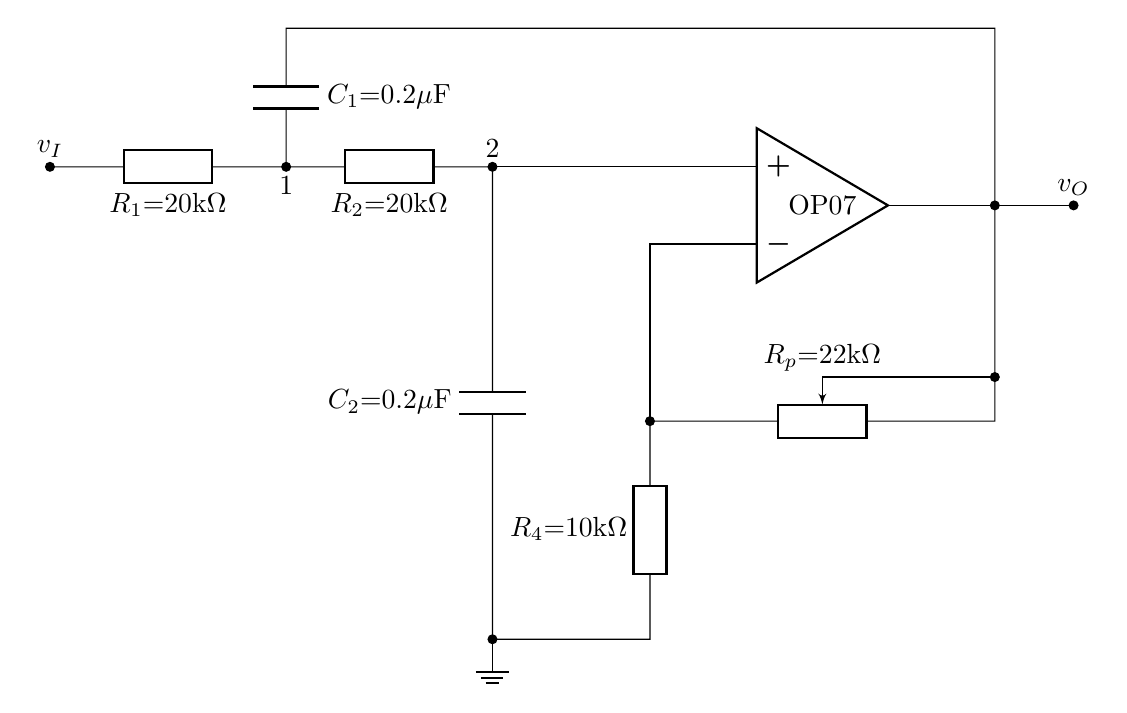
\begin{tikzpicture}[x = 2cm, y = 1.5cm]
\draw (0,0) node[op amp, yscale = -1](AMP){} node{OP07};
\draw (AMP.+) -- ++(-1.5,0) node[circ](N1){} node[anchor = south]{2}
(AMP.-) -| ++(-0.5,-1.5) node[circ](N2){}
(AMP.out) -- ++(0.5,0) node[circ](N3){};

\draw let \p1 = (N1), \p2 = (N2), \p3 = (N3) in
(N2) to [pR, l=$R_p{=}22\text{k}\Omega$, n=PR] ($(\x3,\y2)$) -- (N3) |- ++(-4.5,1.5) to [C, l=$C_1{=}0.2\mu\text{F}$] ($(\x3,\y1)+(-4.5,0)$) node[circ](N4){} node[anchor = north]{1} to [R, l_=$R_2{=}20\text{k}\Omega$] (N1) to [C, l_=$C_2{=}0.2\mu\text{F}$] ++(0,-4) node[circ]{} node[ground]{} -- ++(1,0) to [R, l=$R_4{=}10\text{k}\Omega$] (N2)
;

\draw (N3) -- ++(0.5,0) node[circ]{} node[anchor = south]{$v_O$};
\draw (N4) to [R, l=$R_1{=}20\text{k}\Omega$] ++(-1.5,0) node[circ]{} node[anchor = south]{$v_I$};
\draw let \p1 = (N1), \p2 = (N2), \p3 = (N3) in (PR.wiper) -- ++($(-\x2/2,0)+(\x3/2,0)$) node[circ]{};
\end{tikzpicture}
\caption{有限正增益低通二阶基本节电路图}\label{fig1}
\end{figure}

对节点1、2列电流方程,记节点1的电压为$V_1$,节点2的电压为$V_2$,对同相放大器列电压方程为
\begin{equation}
\begin{array}{c}
(g_1+g_2+sC_1)V_1(s) - g_2V_2(s) - sC_1V_O(s) = g_1V_1(s), \\
-g_2V_1(s) + (g_2+sC_2)V_2(s) = 0, \\
V_O(s) = A_{VF}V_2(s),
\end{array}\label{eq1}
\end{equation}
其中g为电导。由(\ref{eq1})式可得低通二阶基本节传递函数,其一般形式为
\begin{equation}
A(s) = \cfrac{V_O(s)}{V_I} = \cfrac{A_o\omega_L^2}{s^2+\frac{\omega_L}{Q_L}s+\omega_L^2}\label{eq2}
\end{equation}
式中
$$A_o = A_{VF} = 1+\cfrac{R_P}{R_4}$$
$$\omega_L = \cfrac{1}{\sqrt{R_1R_2C_1C_2}}$$
$$Q_L = \cfrac{\sqrt{R_1R_2C_1C_2}}{C_2(R_1+R_2)+R_1C_1(1-A_{VF})}$$
$A_o$为增益,$\omega_L$为特征角频率,$Q_L$为品质因数。在本例中,由于$R_1=R_2=R$、$C_1=C_2=C$,所以有$\omega_L$=1/RC、$Q_L$=1/(3-$A_{VF}$)。其幅频特性为
\begin{equation}
|A_(j\omega)| = \cfrac{A_o}{\sqrt{[1-(\frac{\omega}{\omega_L}^2)]^2 + (\frac{\omega}{\omega_LQ_L})^2}}\label{eq3}
\end{equation}
由此可得其不同Q值的幅频特性曲线,如图(\ref{fig2})。由图(\ref{fig2})可见,若$Q_L$=0.707,则在截止频率$\omega$ = $\omega_L$处,幅频特性下降3dB;称(0,$\omega_L$)为通频带;当$Q_L$=0.707时,通频带内的幅频特性最平坦;当$Q_L>$0.707 时,将出现峰值。由图(\ref{fig2})还可看到,在通频带外,幅频特性曲线是以40dB/十倍频的斜率下降的。

\begin{figure}[!h]
\centering
\includegraphics[width=10cm]{fig/fig2.pdf}\\
\caption{图(\ref{fig1})所示电路的幅频特性}\label{fig2}
\end{figure}

\subsubsection{内容}
\begin{enumerate}
\item 写出$A_o$、$\omega_L$、$Q_L$的灵敏度表达式。例如,$\omega_L$关于$R_1$的灵敏度为
\begin{equation}
S_{R_1}^{\omega_L} = \cfrac{\text{d}\omega_L/\omega_L}{\text{d}R_1/R_1} = \cfrac{R_1}{\omega_L}\cfrac{\text{d}\omega_L}{\text{d}R_1} = -\cfrac{1}{2}\label{eq4}
\end{equation}
\item 调整电路,使其$Q_L$=1,步骤如下。由(\ref{eq2})式可知,在截止频率$f_L$处,其输入-输出相移为$-$90$^{\circ}$。调整输入正弦波信号的频率,使输入-输出相移为$-$90$^{\circ}$,记录信号源的频率,该频率为电路的截止频率$f_L$。由(\ref{eq3})式可知,在截止频率$f_L$处,若$Q_L$=1,则输出幅值为$A_0$;再由(\ref{eq2})式中$Q_L$的表达式可知,在本电路中,由于$R_1$=$R_2$、$C_1$=$C_2$,当$Q_L$=1时, $A_{VF}$=2,即$A_0$=2。再调整$R_p$,使其输出正弦波的幅值为输入的2倍,此时$Q_L$=1。记录$R_p$的阻值。
\item 测量并绘制$Q_L$=1时电路的幅频特性曲线,并与用(\ref{eq3})式绘制的幅频特性曲线做比较。
\end{enumerate}

\subsection{有限正增益高通二阶基本节}
\subsubsection{原理}
图(\ref{fig3})所示电路为有限正增益高通二阶基本节电路。

\begin{figure}[!h]
\centering
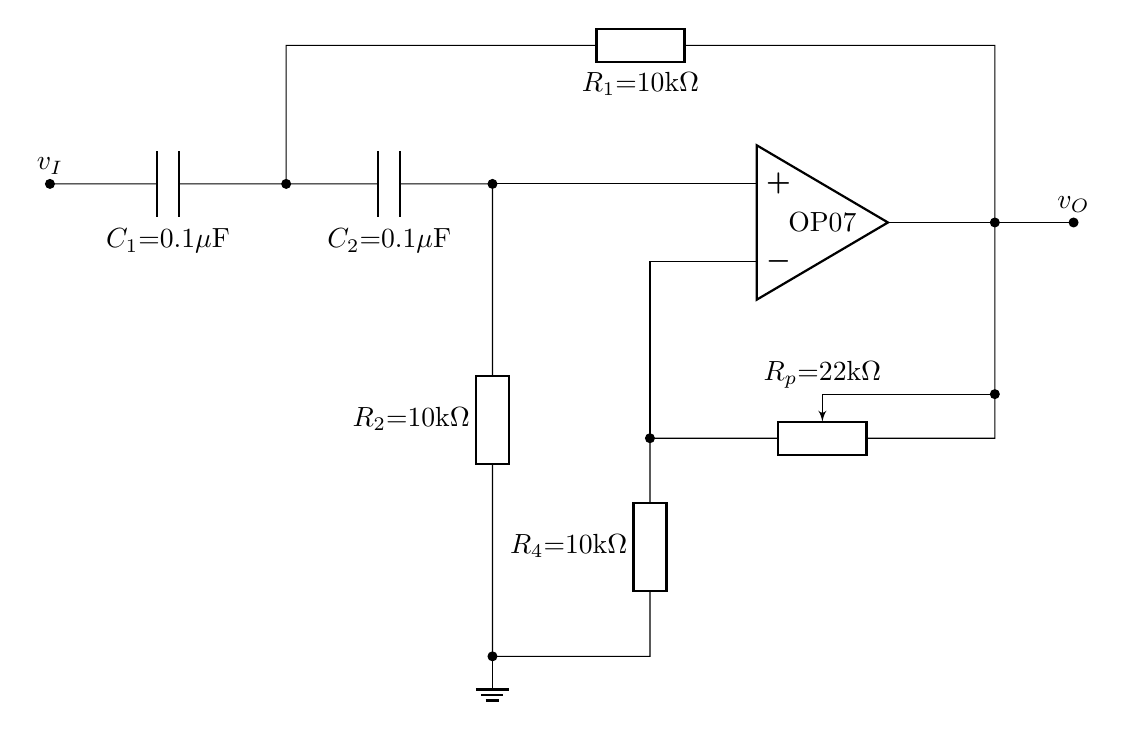
\begin{tikzpicture}[x = 2cm, y = 1.5cm]
\draw (0,0) node[op amp, yscale = -1](AMP){} node{OP07};
\draw (AMP.+) -- ++(-1.5,0) node[circ](N1){}
(AMP.-) -| ++(-0.5,-1.5) node[circ](N2){}
(AMP.out) -- ++(0.5,0) node[circ](N3){};

\draw let \p1 = (N1), \p2 = (N2), \p3 = (N3) in
(N2) to [pR, l=$R_p{=}22\text{k}\Omega$, n=PR] ($(\x3,\y2)$) -- (N3) -- ++(0,1.5) to [R, l=$R_1{=}10\text{k}\Omega$] ++(-4.5,0) -- ($(\x3,\y1)+(-4.5,0)$) node[circ](N4){} to [C, l_=$C_2{=}0.1\mu\text{F}$] (N1) to [R, l_=$R_2{=}10\text{k}\Omega$] ++(0,-4) node[circ]{} node[ground]{} -- ++(1,0) to [R, l=$R_4{=}10\text{k}\Omega$] (N2)
;

\draw (N3) -- ++(0.5,0) node[circ]{} node[anchor = south]{$v_O$};
\draw (N4) to [C, l=$C_1{=}0.1\mu\text{F}$] ++(-1.5,0) node[circ]{} node[anchor = south]{$v_I$};
\draw let \p1 = (N1), \p2 = (N2), \p3 = (N3) in (PR.wiper) -- ++($(-\x2/2,0)+(\x3/2,0)$) node[circ]{};
\end{tikzpicture}
\caption{有限正增益高通二阶基本节电路图}\label{fig3}
\end{figure}

用本节实验(1)的方法可得高通二阶基本节传递函数的一般形式
\begin{equation}
A(s) = \cfrac{V_O(s)}{V_I(s)} = \cfrac{A_os^2}{s^2+\frac{\omega_H}{Q_H}s+\omega_H^2}\label{eq5}
\end{equation}
式中$A_o = A_{VF} = 1+\frac{R_P}{R_4}$,
$$\omega_H = \cfrac{1}{\sqrt{R_1R_2C_1C_2}}\text{, }Q_H = \cfrac{\sqrt{R_1R_2C_1C_2}}{C_1R_1+C_2R_1+R_2C_2(1-A_{VF})}$$
$A_o$为增益,$\omega_H$为特征角频率,$Q_H$为品质因数。在本例中,由于$R_1=R_2=R$、$C_1=C_2=C$,所以有$\omega_H$=1/RC、$Q_H$=1/(3-$A_{VF}$)。其幅频特性为:
\begin{equation}
|A_(j\omega)| = \cfrac{A_o}{\sqrt{[(\frac{\omega_H}{\omega})^2 - 1]^2 + (\frac{\omega_H}{\omega Q_H})^2}}\label{eq6}
\end{equation}
由此可得其不同$Q_H$值的幅频特性曲线,如图(\ref{fig4})。由图(\ref{fig4})可见,若$Q_H$=0.707,则在截止频率$\omega = \omega_H$ 处,幅频特性下降3dB;称$\omega > \omega_H$为通频带;当$Q_H$=0.707时,通频带内的幅频特性最平坦;而当$Q_H>$0.707时,将出现峰值。由图(\ref{fig4})还可看到,在通频带外,幅频特性曲线是以40dB/十倍频的斜率下降的。

\begin{figure}[!h]
\centering
\includegraphics[width=10cm]{fig/fig4.pdf}\\
\caption{图(\ref{fig3})所示电路的幅频特性}\label{fig4}
\end{figure}

\subsubsection{内容}
\begin{enumerate}
\item 写出$A_o$、$\omega_H$、$Q_H$的灵敏度表达式。
\item 调整电路,使其$Q_H$=1,步骤如下。由(\ref{eq5})式可知,在截止频率$f_H$处,其输入-输出相移为90$^{\circ}$。调整输入正弦波信号的频率,使输入-输出相移为90$^{\circ}$,记录信号源的频率,该频率为电路的截止频率$f_H$。由(\ref{eq6})式可知,在截止频率$f_H$处,若$Q_H$=1 ,则输出幅值为$A_o$;再由(\ref{eq5})式中$Q_H$的表达式可知,在本电路中,由于$R_1=R_2$、$C_1=C_2$,当$Q_H$=1时,$A_{VF}$=2,即$A_o$=2。再调整$R_P$,使其输出正弦波的幅值为输入的2倍,此时$Q_H$=1 。记录$R_P$的阻值。
\item 测量并绘制$Q_H$=1时电路的幅频特性曲线,并与用(\ref{eq6})式绘制的幅频特性曲线做比较。
\end{enumerate}

\subsection{有限正增益带通二阶基本节}
\subsubsection{原理}
图(\ref{fig5})所示电路为有限正增益带通二阶基本节电路。

\begin{figure}[!h]
\centering
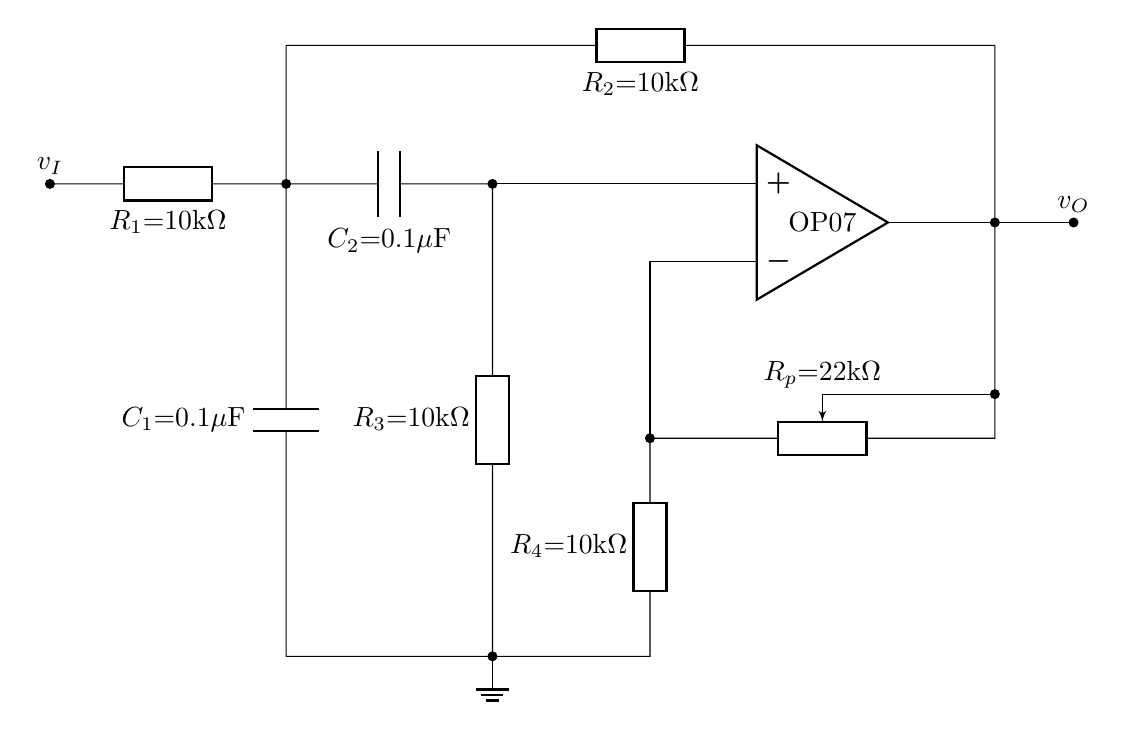
\begin{tikzpicture}[x = 2cm, y = 1.5cm]
\draw (0,0) node[op amp, yscale = -1](AMP){} node{OP07};
\draw (AMP.+) -- ++(-1.5,0) node[circ](N1){}
(AMP.-) -| ++(-0.5,-1.5) node[circ](N2){}
(AMP.out) -- ++(0.5,0) node[circ](N3){};

\draw let \p1 = (N1), \p2 = (N2), \p3 = (N3) in
(N2) to [pR, l=$R_p{=}22\text{k}\Omega$, n=PR] ($(\x3,\y2)$) -- (N3) -- ++(0,1.5) to [R, l=$R_2{=}10\text{k}\Omega$] ++(-4.5,0) -- ($(\x3,\y1)+(-4.5,0)$) node[circ](N4){} to [C, l_=$C_2{=}0.1\mu\text{F}$] (N1) to [R, l_=$R_3{=}10\text{k}\Omega$] ++(0,-4) node[circ](N5){} node[ground]{} -- ++(1,0) to [R, l=$R_4{=}10\text{k}\Omega$] (N2)
;

\draw (N3) -- ++(0.5,0) node[circ]{} node[anchor = south]{$v_O$};
\draw (N4) to [R, l=$R_1{=}10\text{k}\Omega$] ++(-1.5,0) node[circ]{} node[anchor = south]{$v_I$};
\draw let \p1 = (N1), \p2 = (N2), \p3 = (N3) in (PR.wiper) -- ++($(-\x2/2,0)+(\x3/2,0)$) node[circ]{};
\draw let \p1 = (N4), \p2 = (N5) in (N4) to [C, l_=$C_1{=}0.1\mu\text{F}$] ($(\x1,\y2)$) -- (N5);
\end{tikzpicture}
\caption{有限正增益带通二阶基本节电路图}\label{fig5}
\end{figure}

用本节实验(1)的方法可得带通二阶基本节传递函数的一般形式
\begin{equation}
A(s) = \cfrac{V_O(s)}{V_I(s)} = \cfrac{A_o\frac{\omega_P}{Q_P}s}{s^2+\frac{\omega_P}{Q_P}s+\omega_P^2}\label{eq7}
\end{equation}
式中
$$A_o = \cfrac{R_2R_3C_2A_{VF}}{R_1R_2((C_1+C_2)+R_2R_3C_2+R_1R_2R_3(1-A_{VF})}$$
$$\omega_P = \sqrt{\cfrac{R_1+R_2}{R_1R_2R_3C_1C_2}}$$
$$Q_P = \cfrac{\sqrt{R_1+R_2}\sqrt{R_1R_2R_3C_1C_2}}{R_1R_2(C_1+C_2)+R_2R_3C_2+R_1R_3C_2(1-A_{VF})}$$
在本例中,由于$R_1=R_2=R_3=R$、$C_1=C_2=C$,所以有$A_o = \frac{A_{VF}}{4-A_{VF}}$,$\omega_P = \frac{\sqrt{2}}{RC}$,$Q_P = \frac{\sqrt{2}}{4-A_{VF}}$.
其幅频特性为
\begin{equation}
|A_(j\omega)| = \cfrac{A_o}{\sqrt{1+Q_P^2(\frac{\omega_P}{\omega} - \frac{\omega}{\omega_P})^2}}\label{eq8}
\end{equation}
幅频特性曲线如图(\ref{fig6})所示。

\begin{figure}[!h]
\centering
\includegraphics[width=10cm]{fig/fig6.pdf}\\
\caption{图(\ref{fig5})所示电路的幅频特性}\label{fig6}
\end{figure}

通频带带宽为
\begin{equation}
BW = \cfrac{\omega_P}{2\pi Q_P} = \cfrac{f_P}{Q_P}\label{eq9}
\end{equation}
\subsubsection{内容}
\begin{enumerate}
\item 写出$A_o$、$\omega_P$、$Q_P$的灵敏度表达式。
\item 测量其中心频率$f_P$、增益$A_o$。在其中心频率$f_P$处,其输入-输出相移为0$^{\circ}$。调整$R_P$,使$Q_P$=1,即使$f_H - f_L$=$f_P$,$f_H$为上边频,$f_L$为下边频。将$Q_P$=1 、$f_P$、$|A(j\omega)|$=0.707$A_o$代入(\ref{eq8})式,可求出$f_L$、$f_H$,将信号源频率调$f_L$,调整$R_P$,使输出幅值为0.707$A_o$;再将信号源频率调至$f_H$,此时输出幅值应为0.707$A_o$;若不为0.707$A_o$,可微调$R_P$,最终使$f_H - f_L=f_P$。记录$R_P$的阻值。
\item 测量并绘制$Q_P$=1时电路的幅频特性曲线,并与用(\ref{eq8})式绘制的幅频特性曲线比较。
\end{enumerate}

\subsection{单位正增益双T网络带阻二阶基本节}
\subsubsection{原理}
图(\ref{fig7})所示电路为单位正增益双T网络带阻二阶基本节电路。

\begin{figure}[!h]
\centering
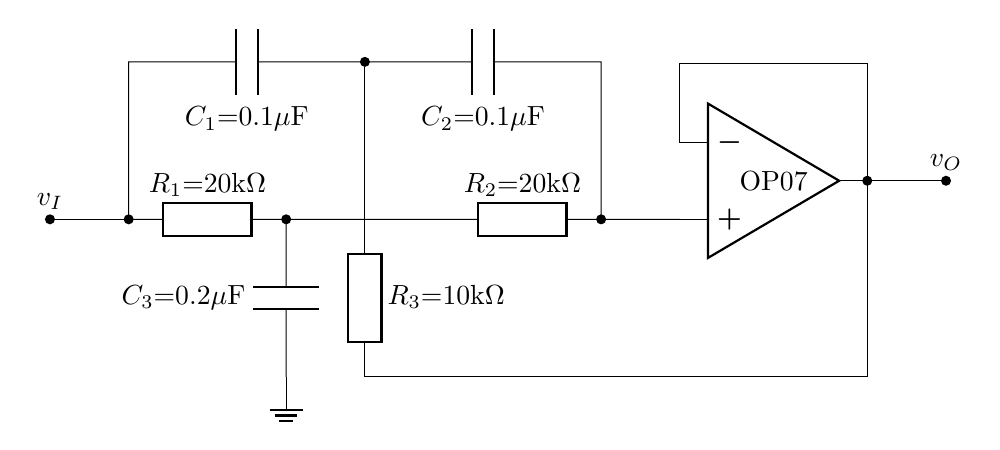
\begin{tikzpicture}[x = 2cm, y = 2cm]
\draw (0,0) node[op amp](AMP){} node{OP07};
\draw (AMP.-) -- ++(0,0.5) -| (AMP.out) node[circ]{};
\draw (AMP.+) -- ++(-0.5,0) node[circ]{} -- ++(0,1) to [C, l=$C_2{=}0.1\mu\text{F}$] ++(-1.5,0) node[circ](T){} to [C, l=$C_1{=}0.1\mu\text{F}$] ++(-1.5,0) -- ++(0,-1) node[circ](OUT){} to [R, l=$R_1{=}20\text{k}\Omega$] ++(1,0) node[circ](N1){} -- ++(1,0) to [R, l=$R_2{=}20\text{k}\Omega$] ++(1,0)
;

\draw (AMP.out) -- ++(0.5,0) node[circ]{} node[anchor = south]{$v_O$};
\draw (OUT) -- ++(-0.5,0) node[circ]{} node[anchor = south]{$v_I$};
\draw (N1) to [C, l_=$C_3{=}0.2\mu\text{F}$] ++(0,-1) node[ground]{};
\draw (T) -- ++(0,-1) to [R, l=$R_3{=}10\text{k}\Omega$] ++(0,-1) -| (AMP.out);
\end{tikzpicture}
\caption{单位正增益双T网络带阻二阶基本节电路图}\label{fig7}
\end{figure}

用本节实验(1)的方法可得带阻二阶基本节传递函数的一般形式为
\begin{equation}
A_(s) = \cfrac{V_O(s)}{V_I(s)} = \cfrac{A_o(s^2+\omega_z^2)}{s^2+\frac{\omega_n}{Q_n}s+\omega_n^2}\label{eq10}
\end{equation}
在电路中,$A_o = A_{VF} = 1$;若$R_1=R_2=2R_3=R$,$C_1=C_2=1/2C_3=C$,则有$\omega_n = \omega_z = \frac{1}{RC}$,$Q_n = \frac{1}{2(2-A_{VF})} = \frac{1}{2}$。其幅频特性曲线如图(\ref{fig8})所示。

\begin{figure}[!h]
\centering
\includegraphics[width=10cm]{fig/fig8.pdf}\\
\caption{图(\ref{fig7})所示电路的幅频特性}\label{fig8}
\end{figure}

\subsubsection{内容}
\begin{enumerate}
\item 测量其幅频特性曲线。求其中心频率(幅值最小时的频率)和中心频率处的增益。
若要求提高电路的品质因数,如何修改图(\ref{fig7}) 所示的电路?试用EWB模拟。
\end{enumerate}

\section{实验数据}
\subsection{有限正增益低通二阶基本节}
测量数据和理论幅频特性曲线如图(\ref{datafig1}):
\begin{figure}[!h]
\centering
\includegraphics[width=10cm]{fig/datafig1.pdf}\\
\caption{低通滤波器幅频特性曲线}\label{datafig1}
\end{figure}

输入信号电压:$V_{irms}$ = 1.0016V,输出信号电压$V_{orms}$ = 2.0032V。得到放大倍数$A_o$ = 2。调节输入信号频率,使相移为$-$90$^{\circ}$,此时输入信号频率为40Hz,滑动变阻器阻值为8.8484k$\Omega$。

$\omega_L$的理论值对应的输入信号频率和理论值与测量值的误差为:
\begin{eqnarray}
f_L &=& \cfrac{\omega_L}{2\pi} = \cfrac{1}{2\pi RC} \approx 39.79\text{ Hz}\label{f_L} \\
\text{Error($f_L$)\%} &=& \cfrac{40 - 39.79}{39.79}\times 100\% \approx 0.53\%
\end{eqnarray}

\subsection{有限正增益高通二阶基本节}
测量数据和理论幅频特性曲线如图(\ref{datafig2}):
\begin{figure}[!h]
\centering
\includegraphics[width=10cm]{fig/datafig2.pdf}\\
\caption{高通滤波器幅频特性曲线}\label{datafig2}
\end{figure}

输入信号电压:$V_{irms}$ = 1.0035V,输出信号电压$V_{orms}$ = 2.0070V。得到放大倍数$A_o$ = 2。调节输入信号频率,使相移为90$^{\circ}$,此时输入信号频率为158Hz,滑动变阻器阻值为9.85859k$\Omega$。

$\omega_H$的理论值对应的输入信号频率和理论值与测量值的误差为:
\begin{eqnarray}
f_H &=& \cfrac{\omega_H}{2\pi} = \cfrac{1}{2\pi RC} \approx 159.15\text{ Hz} \\
\text{Error($f_H$)\%} &=& \cfrac{158 - 159.15}{159.15}\times 100\% \approx -0.72\%
\end{eqnarray}
\subsection{有限正增益带通二阶基本节}
测量数据和理论幅频特性曲线如图(\ref{datafig3}):
\begin{figure}[!h]
\centering
\includegraphics[width=10cm]{fig/datafig3.pdf}\\
\caption{带通滤波器幅频特性曲线}\label{datafig3}
\end{figure}

输入信号电压:$V_{irms}$ = 1.003V,输出信号电压$V_{orms}$ = 1.834V。得到放大倍数$A_o$ = 1.8285。调节输入信号频率,使相移为0$^{\circ}$,此时输入信号频率为222Hz,滑动变阻器的阻值为15.6398k$\Omega$。

测得的通频带上下截止频率分别为:
$$f_{PL}\text{ = 138.64}Hz$$
$$f_{PH}\text{ = 355.31Hz}$$
计算得到品质因子为:
\begin{equation}
Q = \cfrac{f_P}{f_{PH} - f_{PL}} \approx 1.0246
\end{equation}

$\omega_P$的理论值对应的输入信号频率和理论值与测量值的误差为:
\begin{eqnarray}
f_P &=& \cfrac{\omega_P}{2\pi} = \cfrac{1}{2\pi RC} \approx 225.08\text{ Hz}\label{f_P} \\
\text{Error($f_P$)\%} &=& \cfrac{222 - 225.08}{225.08}\times 100\% \approx -1.37\%
\end{eqnarray}
\subsection{单位正增益双T网络带阻二阶基本节}
测量数据和理论幅频特性曲线如图(\ref{datafig4}):
\begin{figure}[!h]
\centering
\includegraphics[width=10cm]{fig/datafig4.pdf}\\
\caption{带阻滤波器幅频特性曲线}\label{datafig4}
\end{figure}

输出信号电压最小时的输入信号频率为77.5Hz,理论值为:
\begin{equation}
f_n = \cfrac{\omega_n}{2\pi} = \cfrac{1}{2\pi RC} \approx 79.58\text{ Hz}
\end{equation}

误差为:
\begin{equation}
\text{Error($f_n$)\%} = \cfrac{77.5 - 79.58}{79.58}\times 100\% \approx -0.03\%
\end{equation}

\section{实验讨论}
\iffalse
\subsection{电容位置与高通、低通滤波器}
在图(\ref{fig1})中,电容接地意味着高频信号直接到地,输入运放的是低频信号,因此为低通滤波器;图(\ref{fig3})中电容在前,输入信号中只有高频信号能通过并到达运放,因此为高通滤波器。
\fi

\section{思考题}
%\subsection{在图(\ref{fig1})中,改变$R_P$,由实验找出该电路可能达到最大的品质因数。试述实测值与理论计算值有差别的原因。}
%\subsection{图(\ref{fig1})中,改变$R_P$,若使$R_P$大于20k$\Omega$,电路会发生什么情况?试从理论上给予说明。}
\subsection{在图(\ref{fig1})中,当$Q_L$=1时,为了寻找截止频率为什么观察相位而不观察幅值?}

\nocite{jiaocai}
%--------bib------------------
\bibliography{ref}
\end{document}